% Paper 1: Knowledge Graph Quality Assessment and Enhancement
% Focus: Innovation 1 (Quality Aggregation Model) + Innovation 3 (Multi-dimensional Analysis Framework)

\documentclass[runningheads]{llncs}
\usepackage[T1]{fontenc}
\usepackage{graphicx}
\usepackage{times}
\usepackage{latexsym}
\usepackage{amsmath}
\usepackage{amsfonts}
\usepackage{booktabs}
\usepackage{multirow}
\usepackage{tabularx}
\usepackage{float}
\usepackage{makecell}
\usepackage{geometry}
\geometry{margin=1in}
\usepackage{pgfplots}
\usepackage{tikz}
\pgfplotsset{compat=1.18}
\usepackage{pgfplotstable}

% Custom color palette
\definecolor{myblue}{RGB}{52, 114, 186}
\definecolor{myorange}{RGB}{220, 110, 40}
\definecolor{mygreen}{RGB}{48, 148, 86}
\definecolor{myteal}{RGB}{42, 148, 160}
\definecolor{mypurple}{RGB}{130, 92, 168}

\pgfplotsset{
    every axis/.append style={
        width=\textwidth,
        height=7cm,
        grid=major,
        grid style={dashed, gray!20},
        legend pos=north west,
        legend style={
            font=\small,
            draw=gray!50,
            fill=white,
            rounded corners=2pt,
            inner sep=5pt,
        },
        label style={font=\small},
        tick label style={font=\small},
        axis line style={gray!60},
        tick style={draw=none},
        axis background/.style={fill=gray!4},
        axis lines=left,
        enlarge x limits=0.1,
    }
}
\usepackage[utf8]{inputenc}
\usepackage{microtype}
\usepackage{inconsolata}

\begin{document}

\title{Constraint-Based Knowledge Graph Quality Enhancement: A Multi-Strategy Framework for Comprehensive Quality Optimization}

\titlerunning{Constraint-Based KG Quality Enhancement}

\author{\inst{1} \and
\inst{2}}

\authorrunning{ et al.}

\institute{
\email{} \and
\\
\email{}}

\maketitle

\begin{abstract}
Knowledge graph (KG) construction faces critical challenges in quality assurance when dealing with low-quality, inconsistent data. Existing methods rely on single-dimensional metrics or lack systematic enhancement mechanisms. This paper proposes a constraint-based framework that formulates KG quality assessment as an optimization problem across four orthogonal dimensions: node connectivity, triple uniqueness, logical consistency, and semantic soundness. We introduce: (1) a constrained hierarchical quality aggregation model with hard constraint optimization ensuring critical indicators meet minimum thresholds while balancing inter-dimensional trade-offs; (2) a multi-strategy collaborative analysis framework combining detail-oriented, global-oriented, and behavior simulation strategies for targeted defect repair. Experiments across government, finance, and environment domains demonstrate that our system improves KG quality scores by 8.89 points on low-quality data, significantly outperforming rule-based (+7.14) and LLM-only (+4.46) baselines. Ablation studies confirm synergistic benefits (+2.30) from multi-strategy integration. Results show strong cross-domain generalization and robustness to data quality degradation.

\keywords{Knowledge Graph Construction \and Quality Assessment \and Constrained Optimization \and Multi-Strategy Enhancement \and Large Language Models}
\end{abstract}

\section{Introduction}

\subsection{Research Background and Motivation}
With the advancement of digital transformation, the global data volume is growing at an unprecedented rate, of which more than 80\% consists of unstructured or semi-structured text. How to efficiently and accurately extract valuable knowledge from such massive data and convert it into a machine-understandable and machine-reasonable format has become a core issue in advancing artificial intelligence from perceptual intelligence to cognitive intelligence. Knowledge Graph (KG), as a large-scale semantic network that organizes and stores human knowledge in the form of structured triples ($\langle$Subject, Relation, Object$\rangle$), provides an excellent interface for automated machine reading, analysis, and processing.

However, constructing a high-quality, large-scale knowledge graph faces critical bottlenecks at multiple levels:

\begin{enumerate}
    \item \textbf{Structural level challenges}: Text data in the real world is often incomplete, leading to fragmented graphs with isolated nodes and redundant information. Most construction methods lack mechanisms for optimizing graph topology and connectivity.
    \item \textbf{Logical level challenges}: Existing quality assessment methods focus on isolated metrics without considering interdependencies and constraint violations. Domain-specific logical rules are often violated, leading to inconsistent hierarchies and type conflicts.
    \item \textbf{Semantic level challenges}: Current repair techniques are primarily rule-based with limited coverage, unable to address complex semantic errors and factual incorrectness in a holistic manner. LLM-based methods suffer from hallucinations and lack systematic validation.
    \item \textbf{Lack of multi-level integration}: No existing framework systematically addresses quality issues across all three levels (structural, logical, semantic) in a unified manner.
\end{enumerate}

\subsection{Contributions of This Paper}
To address these challenges, this paper proposes a comprehensive knowledge graph quality assessment and enhancement framework based on constrained optimization and multi-strategy collaboration. The main contributions are:

\begin{enumerate}
    \item \textbf{Constrained Optimization Model for Quality Aggregation}: We formulate KG quality assessment as a constrained optimization problem that simultaneously optimizes four orthogonal dimensions (node connectivity, triple uniqueness, logical consistency, and semantic soundness) while enforcing hard constraints on critical indicators. This principled approach ensures that quality improvements in one dimension do not degrade others, and that essential properties (e.g., logical consistency) always meet minimum thresholds. Unlike prior work that treats dimensions independently, our model captures inter-dimensional trade-offs and provides a unified optimization objective.

    \item \textbf{Multi-Strategy Collaborative Enhancement Framework}: We design a three-strategy analysis framework (detail-oriented, global-oriented, and behavior simulation) that operates at different granularities to identify defects across structural, logical, and semantic levels. Each strategy targets specific defect types: detail-oriented analysis addresses local structural issues, global-oriented analysis detects logical patterns and constraint violations, and behavior simulation validates semantic correctness through process modeling. Combined with a comprehensive completion engine integrating web search, LLM reasoning, and rule-based inference, this framework achieves targeted enhancement across all quality dimensions.

    \item \textbf{Empirical Validation on Low-Quality Data}: Through extensive experiments on systematically degraded datasets across three domains, we demonstrate that our constraint-based approach significantly outperforms pure rule-based (+7.14 points) and pure LLM-based (+4.46 points) methods. Ablation studies confirm that multi-strategy integration provides synergistic benefits (+2.30 points) beyond any single strategy, validating the effectiveness of our holistic approach.
\end{enumerate}

Extensive experiments conducted in three vertical domains (government affairs, finance, and environment) verify the effectiveness and robustness of the proposed framework. Experimental results show that the comprehensive quality score improves by an average of 8.89 points, with semantic soundness improving by 16.56 points and logical consistency by 8.35 points.

\subsection{Paper Organization}
The rest of this paper is organized as follows: Section 2 reviews related work on KG construction, quality assessment, and enhancement methods. Section 3 elaborates on the proposed multi-level quality assessment model and hierarchical enhancement framework. Section 4 presents experimental design and results demonstrating effectiveness across structural, logical, and semantic levels. Section 5 concludes the paper and discusses future directions.

\section{Related Work}
\label{sec:related_work}

\subsection{Knowledge Graph Construction Methods}

\subsubsection{Traditional Rule-Based Approaches}
Traditional KG construction primarily follows a pipeline of data extraction, entity linking, relationship mapping, and graph assembly \cite{ref_ji2021}. Early foundational systems rely on structured data sources and rule-based logic: DBpedia \cite{ref_auer2007} parses Wikipedia infoboxes to generate over 4.5 billion triples, while YAGO \cite{ref_suchanek2007} integrates WordNet ontologies to ensure hierarchical consistency. Freebase \cite{ref_bollacker2008} provides a collaborative platform for structured knowledge curation. However, these methods face limitations in scalability, high labor costs for rule curation, and error propagation from flawed extraction logic \cite{ref_dong2014}.

\subsubsection{Neural and Embedding-Based Methods}
With the rise of deep learning, neural approaches have been applied to KG construction tasks. TransE \cite{ref_bordes2013} and its variants model entities and relations as embeddings in continuous vector spaces for link prediction. Graph neural networks (GNNs) \cite{ref_schlichtkrull2018} leverage neighborhood information for entity classification and relation extraction. These methods improve scalability but often lack interpretability and struggle with rare entities \cite{ref_wang2017}.

\subsubsection{LLM-Based Knowledge Engineering}
Large Language Models (LLMs) have revolutionized KG construction through end-to-end Text-to-KG pipelines \cite{ref_zhang2023}. Zero-shot/few-shot prompting extracts triples via natural language instructions \cite{ref_wei2023}, while fine-tuning optimizes LLMs on domain-specific datasets for higher accuracy \cite{ref_pan2024}. Knowledge fusion combines LLM-extracted implicit knowledge with structured KGs to mitigate hallucinations \cite{ref_pan2023}. Recent work explores prompt engineering strategies \cite{ref_white2023} and retrieval-augmented generation \cite{ref_lewis2020} to improve extraction quality. However, challenges persist including hallucinations, limited cross-domain generalization, and high computational demands \cite{ref_ji2023}.

\subsection{Knowledge Graph Quality Assessment}

\subsubsection{Quality Dimensions and Metrics}
KG quality is evaluated across multiple dimensions. Zaveri et al. \cite{ref_zaveri2016} propose a comprehensive taxonomy including accuracy, completeness, consistency, and timeliness. Paulheim \cite{ref_paulheim2017} surveys quality assessment methods focusing on intrinsic metrics (e.g., consistency) and extrinsic metrics (e.g., task performance). Wang et al. \cite{ref_wang2021} emphasize the importance of domain-specific quality criteria and user-centric evaluation.

\subsubsection{Automated Quality Assessment}
Automated assessment techniques leverage statistical and machine learning methods. Embedding-based approaches \cite{ref_nickel2016} score triple plausibility using learned representations. Rule-based validators \cite{ref_kontokostas2014} detect violations of logical constraints. Hybrid methods \cite{ref_paulheim2014} combine multiple signals for comprehensive quality scoring. Recent work explores LLM-based semantic evaluation \cite{ref_lin2025} for fine-grained quality assessment.

\subsection{Knowledge Graph Quality Enhancement and Repair}

\subsubsection{Error Detection and Correction}
Error detection methods identify inconsistencies, incompleteness, and inaccuracies in KGs. Statistical outlier detection \cite{ref_wienand2014} flags anomalous triples. Constraint-based validation \cite{ref_kontokostas2014} checks compliance with ontological rules. Crowdsourcing approaches \cite{ref_acosta2013} leverage human judgment for error identification. Correction techniques include rule-based repair \cite{ref_paulheim2014}, embedding-based completion \cite{ref_shi2017}, and LLM-driven reasoning \cite{ref_lin2025}.

\subsubsection{Knowledge Graph Completion}
KG completion aims to infer missing facts. Path-based methods \cite{ref_lao2011} use relational paths for inference. Embedding methods \cite{ref_bordes2013,ref_yang2015} predict missing links in latent space. Neural approaches \cite{ref_dettmers2018} leverage convolutional and recurrent architectures. Recent work explores reinforcement learning \cite{ref_das2018} and meta-learning \cite{ref_chen2019} for adaptive completion strategies.

\subsubsection{Hierarchical and Multi-dimensional Enhancement}
While existing methods address specific quality issues, few provide systematic frameworks for multi-level enhancement. Table \ref{tab:related_work_comparison} compares our approach with representative prior work.

\begin{table}[H]
    \centering
    \caption{Comparison with Related Work on KG Quality Enhancement}
    \label{tab:related_work_comparison}
    \begin{tabular}{p{3cm} p{2cm} p{2.5cm} p{1.5cm} p{2cm}}
    \toprule
    \textbf{Method} & \textbf{Quality Dimensions} & \textbf{Enhancement Strategy} & \textbf{Uses LLM} & \textbf{Cross-Domain} \\
    \midrule
    Paulheim \cite{ref_paulheim2014} & Consistency & Statistical repair & No & Limited \\
    Shi et al. \cite{ref_shi2017} & Completeness & Embedding-based & No & Yes \\
    Lin et al. \cite{ref_lin2025} & Semantic & LLM reasoning & Yes & Limited \\
    \textbf{Our Method} & \textbf{All 4 dimensions} & \textbf{Constraint optimization + Multi-strategy} & \textbf{Yes} & \textbf{Yes} \\
    \bottomrule
    \end{tabular}
\end{table}

Our work differs by: (1) addressing all four quality dimensions simultaneously through constrained optimization rather than treating them independently; (2) providing a principled framework that integrates structural, logical, and semantic enhancement strategies; (3) demonstrating robust cross-domain performance on low-quality data.

\section{Methodology}

\subsection{Framework Overview}
Our multi-level framework systematically enhances KG quality through three hierarchical levels: structural, logical, and semantic. The framework consists of three integrated components: (1) a constrained hierarchical quality aggregation model for comprehensive assessment across all levels, (2) a multi-dimensional collaborative analysis framework for defect identification at each level, and (3) a comprehensive completion engine for targeted enhancement. The system processes input text through initial KG construction, multi-level quality assessment, and iterative enhancement until quality thresholds are met at all levels.

\begin{figure}
    \centering
    \includegraphics[width=1.0\linewidth]{image.png}
    \caption{Framework Overview}
    \label{fig:placeholder}
\end{figure}

We decompose the quality $Q$ of a knowledge graph into four primary indicators that span three hierarchical levels: structural level (node connectivity, triple uniqueness), logical level (logical consistency), and semantic level (semantic soundness).

\subsubsection{Level 1: Structural Quality Metrics}

\paragraph{1. Node Connectivity}
\textbf{Physical Meaning:} Connectivity measures the organizational efficiency at the macro-structural level and the density of knowledge associations at the micro level. A high-quality KG should be an effectively interconnected network, not isolated knowledge islands.

\textbf{Quantitative Indicators:} We use graph-theoretic metrics to quantify connectivity $S(C_1)$:
\begin{itemize}
    \item \textit{Isolated Node Rate ($I_r$)}: Proportion of nodes without connections
    \item \textit{Average Degree ($\bar{d}$)}: Overall density of the knowledge graph
    \item \textit{Clustering Coefficient ($C_c$)}: Tightness of interconnections between neighboring nodes
\end{itemize}

\paragraph{2. Triple Uniqueness}
\textbf{Physical Meaning:} Uniqueness measures information efficiency and signal-to-noise ratio. Redundant triples increase information entropy and reduce knowledge representation conciseness.

\textbf{Quantitative Indicators:} We use the Redundant Triple Rate ($R_r$):
\begin{equation}
\label{eq:uniqueness_score}
S(C_2) = 1 - R_r
\end{equation}

\subsubsection{Level 2: Logical Quality Metrics}

\paragraph{3. Logical Consistency}
\textbf{Physical Meaning:} Logical consistency ensures trustworthiness and reliability at the constraint satisfaction level. A KG with logical contradictions cannot support rigorous reasoning and decision-making.

\textbf{Quantitative Indicators:} We quantify logical consistency $S(C_3)$ based on domain rules:
\begin{equation}
\label{eq:consistency_score}
S(C_3) = 1 - (w_1 T_c + w_2 H_c)
\end{equation}
where $T_c$ is type conflict rate and $H_c$ is hierarchical conflict rate.

\subsubsection{Level 3: Semantic Quality Metrics}

\paragraph{4. Semantic Soundness}
\textbf{Physical Meaning:} Semantic soundness measures whether facts conform to the real world and are applicable to specific domains at the highest level of abstraction.

\textbf{Quantitative Indicators:} We use LLM-based evaluation:
\begin{equation}
\label{eq:semantic_score}
S(C_4) = \frac{1}{K} \sum_{k=1}^{K} s_k
\end{equation}
where $K$ is the number of sampled triples and $s_k$ is the LLM-assigned score.

\subsubsection{Constrained Optimization Formulation}
The comprehensive quality score $Q(G)$ is defined as:
\begin{equation}
\label{eq:kg_quality_optimization}
\begin{cases}
\max_{G} \quad Q(G) = \sum_{i=1}^{4} w_i S(C_i) \\
\text{s.t.} \quad
\begin{cases}
S(C_3) \ge \theta_{\text{consistency}} & \text{(Hard Constraint)} \\
\theta_{\text{min\_conn}} \le S(C_1) \le \theta_{\text{max\_conn}} & \text{(Balance Constraint)} \\
S(C_2) \ge \theta_{\text{uniqueness}} & \text{(Optional Constraint)} \\
S(C_4) \ge \theta_{\text{semantic}} & \text{(Optional Constraint)}
\end{cases}
\end{cases}
\end{equation}
where $w_i$ are importance weights ($w_1=0.2$, $w_2=0.2$, $w_3=0.3$, $w_4=0.3$).

\subsection{Multi-dimensional Collaborative Analysis Framework for Graph Enhancement}
\label{subsec:enhancement_framework}

This framework serves as the core mechanism for identifying and repairing KG defects across all three hierarchical levels. It comprehensively identifies deficiencies through three analysis types that operate at different granularities, each targeting specific quality levels.

\begin{figure}
    \centering
    
\includegraphics[width=1.0\linewidth]{image2.png}
    \caption{Multi-Strategy Collaborative Analysis Framework}
    \label{fig:placeholder}
\end{figure}

\subsubsection{Detail-Oriented Analysis: Structural Level Defect Detection}

Detail-oriented analysis focuses on local structural issues by examining individual entities and their immediate neighborhoods. This bottom-up approach targets structural-level quality problems:

\paragraph{Isolated Node Detection}
We identify disconnected entities that lack incoming or outgoing edges:
\begin{equation}
\text{Isolated}(e) = \begin{cases}
1 & \text{if } \deg(e) = 0 \\
0 & \text{otherwise}
\end{cases}
\end{equation}
where $\deg(e)$ is the degree of entity $e$. For each isolated node, we analyze the source text to identify missing relationships through:
\begin{itemize}
    \item \textit{Co-occurrence analysis}: Entities mentioned in the same sentence or paragraph likely share relationships
    \item \textit{Syntactic dependency parsing}: Extract subject-verb-object patterns to infer missing edges
    \item \textit{Attribute completeness checking}: Verify that essential attributes (e.g., type, description) are present
\end{itemize}

\paragraph{Redundancy Detection}
We detect duplicate or near-duplicate triples through semantic similarity scoring. Given two triples $t_1 = (s_1, r_1, o_1)$ and $t_2 = (s_2, r_2, o_2)$, we compute:
\begin{equation}
\text{Sim}(t_1, t_2) = \alpha \cdot \text{cos}(\mathbf{e}_{s_1}, \mathbf{e}_{s_2}) + \beta \cdot \text{cos}(\mathbf{e}_{r_1}, \mathbf{e}_{r_2}) + \gamma \cdot \text{cos}(\mathbf{e}_{o_1}, \mathbf{e}_{o_2})
\end{equation}
where $\mathbf{e}_x$ denotes the embedding of element $x$, and $\alpha + \beta + \gamma = 1$ (we use $\alpha=0.4, \beta=0.2, \gamma=0.4$). Triples with $\text{Sim}(t_1, t_2) > \tau_{\text{dup}}$ (threshold $\tau_{\text{dup}}=0.85$) are marked as redundant.

\paragraph{Type Conflict Detection}
We check entity type consistency by validating that entity types align with their relationships:
\begin{equation}
\text{TypeValid}(s, r, o) = \text{Compatible}(\text{Type}(s), \text{Domain}(r)) \land \text{Compatible}(\text{Type}(o), \text{Range}(r))
\end{equation}

\subsubsection{Global-Oriented Analysis: Logical Level Pattern Recognition}

Global-oriented analysis examines the entire graph structure to identify logical patterns and constraint violations. This top-down approach targets logical-level quality issues:

\paragraph{Hierarchical Consistency Checking}
We validate hierarchical relationships (e.g., organizational structures, taxonomies) by checking transitivity and acyclicity:
\begin{itemize}
    \item \textit{Transitivity validation}: If $A \prec B$ and $B \prec C$, then $A \prec C$ should hold
    \item \textit{Cycle detection}: Hierarchical relations must form a directed acyclic graph (DAG)
    \item \textit{Level consistency}: Entities at the same hierarchical level should have similar properties
\end{itemize}

\paragraph{Statistical Pattern Analysis}
We leverage statistical features to identify anomalies. For each entity $e$, we compute its z-score based on degree distribution:
\begin{equation}
z(e) = \frac{\deg(e) - \mu_{\deg}}{\sigma_{\deg}}
\end{equation}
where $\mu_{\deg}$ and $\sigma_{\deg}$ are the mean and standard deviation of node degrees. Entities with $|z(e)| > 3$ are flagged for manual inspection as potential anomalies.

\paragraph{Rule-Based Validation}
We apply domain-specific logical rules to detect violations:
\begin{itemize}
    \item \textit{Cardinality constraints}: E.g., a person can have at most one birthdate
    \item \textit{Domain constraints}: E.g., a "manages" relation requires both subject and object to be organizational entities
    \item \textit{Temporal constraints}: E.g., event start time must precede end time
\end{itemize}

\subsubsection{Behavior Simulation Analysis: Semantic Level Validation}

Behavior simulation analysis validates semantic correctness by simulating real-world processes and checking if the KG supports them. This approach targets semantic-level quality:

\paragraph{Process Simulation}
For procedural knowledge (e.g., administrative workflows, manufacturing processes), we simulate execution:
\begin{enumerate}
    \item \textit{Step extraction}: Identify sequential steps from the source text
    \item \textit{Precondition checking}: Verify that each step's preconditions are satisfied by previous steps
    \item \textit{Resource validation}: Ensure required entities (actors, objects) exist and are accessible
    \item \textit{Outcome verification}: Check that expected outcomes are represented in the KG
\end{enumerate}

\paragraph{Causal Chain Validation}
We verify causal relationships by checking logical consistency:
\begin{itemize}
    \item \textit{Cause-effect pairs}: Validate that causes temporally precede effects
    \item \textit{Causal transitivity}: If $A$ causes $B$ and $B$ causes $C$, check if $A \rightarrow C$ is implied
    \item \textit{Counterfactual reasoning}: Use LLM to assess whether removing a cause would eliminate the effect
\end{itemize}

\paragraph{LLM-Based Semantic Scoring}
We employ LLMs to assess factual correctness and domain appropriateness:
\begin{itemize}
    \item \textit{Factual verification}: Query LLM to verify if triples align with world knowledge
    \item \textit{Domain consistency}: Check if terminology and relationships are appropriate for the domain
    \item \textit{Contextual plausibility}: Assess whether triples make sense given surrounding context
\end{itemize}

\subsubsection{Comprehensive Completion Engine}

The completion engine integrates three methods that target different enhancement levels:

\paragraph{Web Search Completion (Structural + Semantic)}
For missing attributes or relationships, we query external knowledge sources:
\begin{enumerate}
    \item \textit{Query formulation}: Generate search queries from entity names and context
    \item \textit{Source retrieval}: Fetch authoritative sources (e.g., official websites, databases)
    \item \textit{Information extraction}: Extract relevant facts using NER and relation extraction
    \item \textit{Validation}: Cross-check extracted information with existing KG content
\end{enumerate}

\paragraph{Inferential Completion (Logical + Semantic)}
For implicit relationships, we use LLM reasoning:
\begin{enumerate}
    \item \textit{Context assembly}: Gather relevant triples and source text as context
    \item \textit{Reasoning prompt}: Construct prompts that guide LLM to infer missing information
    \item \textit{Confidence scoring}: Assess confidence of inferred facts
    \item \textit{Consistency checking}: Verify inferred facts don't contradict existing knowledge
\end{enumerate}

\paragraph{Rule Set Completion (Logical)}
For domain-specific knowledge, we apply rule-based completion:
\begin{enumerate}
    \item \textit{Rule matching}: Identify applicable rules based on entity types and relations
    \item \textit{Template instantiation}: Fill rule templates with specific entities
    \item \textit{Constraint propagation}: Derive new facts through logical inference
    \item \textit{Validation}: Ensure generated facts satisfy all constraints
\end{enumerate}

\subsubsection{Multi-Level Integration Strategy}

The three analysis strategies work collaboratively in an iterative refinement loop:
\begin{enumerate}
    \item \textit{Initial pass}: Detail-oriented analysis identifies local structural issues
    \item \textit{Pattern recognition}: Global-oriented analysis detects logical inconsistencies
    \item \textit{Semantic validation}: Behavior simulation verifies factual correctness
    \item \textit{Iterative refinement}: Repeat until quality thresholds are met at all levels
\end{enumerate}

This multi-level integration ensures that improvements at one level don't degrade quality at other levels, achieving holistic optimization.

\section{Experiments}

\subsection{Experimental Setup}

\subsubsection{Datasets}
We evaluate our framework on three real-world administrative datasets spanning government affairs, finance, and environmental regulation. These domains are deliberately chosen to reflect heterogeneous quality challenges: government affairs documents exhibit complex organizational hierarchies prone to relational conflicts, financial regulatory texts are dense with domain-specific terminology that is sensitive to semantic errors, and environmental documents combine procedural workflows with multi-level agency structures. Together, they allow us to assess whether the proposed multi-level framework generalizes beyond any single domain characteristic.

\begin{table}[H]
    \centering
    \caption{Statistical Information of Experimental Datasets}
    \label{tab:dataset_stats}
    \begin{tabularx}{\textwidth}{l l X}
    \toprule
    Domain & Sample Size & Data Source \\
    \midrule
    Government Affairs & 2,100 entries & Shaanxi Provincial Government Website \\
    Finance & 500 entries & National Financial Regulatory Administration \\
    Environment & 500 entries & Ministry of Ecology and Environment \\
    \bottomrule
    \end{tabularx}
\end{table}

To simulate realistic degradation conditions, we constructed low-quality counterparts through controlled injection of quality issues. The degradation categories were derived from an analysis of common error patterns reported in prior KG quality studies~\cite{ref_zaveri2016,ref_paulheim2017}, ensuring ecological validity. Each issue type was injected independently to enable targeted evaluation of individual enhancement components. The resulting degradation rates (Table~\ref{tab:degradation_stats}) vary across domains, reflecting the distinct structural properties of each dataset rather than uniform artificial corruption.

\begin{table}[H]
    \centering
    \caption{Degradation Strategies and Statistics}
    \label{tab:degradation_stats}
    \begin{tabularx}{\textwidth}{l c c c X}
    \toprule
    Quality Issue Type & Gov & Finance & Env & Strategy \\
    \midrule
    Field Missing & 26.5\% & 11.7\% & 11.6\% & Delete key fields \\
    Information Inconsistency & 26.5\% & 10.2\% & 10.2\% & Conflicts in dates/amounts \\
    Terminology Error & 25.6\% & 11.3\% & 11.8\% & Replace with incorrect terms \\
    Logical Contradiction & 27.1\% & 11.0\% & 11.8\% & Hierarchical errors \\
    Relationship Error & 27.9\% & 13.2\% & 9.8\% & Subject-object reversal \\
    Hierarchical Conflict & 37.6\% & 21.5\% & 23.0\% & Subordinate managing superior \\
    \bottomrule
    \end{tabularx}
\end{table}

\subsubsection{Experimental Design}
Our experimental design is structured to answer three research questions: (RQ1) Does our full framework effectively recover quality from degraded KGs? (RQ2) What is the relative contribution of each hierarchical level? (RQ3) How does the framework compare against simpler single-strategy baselines?

To address these questions, we define eight experimental configurations (Table~\ref{tab:exp_design}). Exp~1 establishes the quality ceiling by processing clean data, providing a reference for what an uncompromised KG looks like under our metrics. Exp~2 applies no enhancement to the degraded data, measuring the severity of quality degradation and setting the lower bound that our system must improve upon. Exp~3 applies the full system and is our primary result. Exps~4--6 are ablation variants that isolate the contribution of each individual level; crucially, these reveal not only how much each level contributes, but \textit{which types of defects} each level addresses, allowing us to validate the design rationale of the three-level hierarchy. Exps~7--8 serve as comparative baselines representing common simpler strategies: rule-based only and LLM-only enhancement, both of which lack the multi-level integration that our framework provides.

\begin{table}[H]
    \centering
    \caption{Experimental Design Matrix}
    \label{tab:exp_design}
    \small
    \begin{tabular}{l l p{6cm}}
    \toprule
    \textbf{Exp ID} & \textbf{Data Type} & \textbf{Objective} \\
    \midrule
    Exp 1 & Normal & Baseline (ideal conditions) \\
    Exp 2 & Low-Quality & Impact assessment \\
    Exp 3 & Low-Q + Full & Full system effectiveness \\
    Exp 4 & Low-Q + Struct & Structural contribution \\
    Exp 5 & Low-Q + Logic & Logical contribution \\
    Exp 6 & Low-Q + Sem & Semantic contribution \\
    Exp 7 & Low-Q + Rules & Rule-based baseline \\
    Exp 8 & Low-Q + LLM & LLM-only baseline \\
    \bottomrule
    \end{tabular}
\end{table}

\subsubsection{Evaluation Metrics}
We evaluate quality across four dimensions, each corresponding to a distinct type of KG defect:
\begin{itemize}
    \item \textit{Isolation Score ($S_{iso}$)}: $(1 - \text{isolated node rate}) \times 100$
    \item \textit{Redundancy Score ($S_{red}$)}: $(1 - \text{redundant triple rate}) \times 100$
    \item \textit{Logic Score ($S_{log}$)}: $(1 - \text{logical conflict rate}) \times 100$
    \item \textit{Semantic Score ($S_{sem}$)}: $\text{LLM evaluation score} \times 100$
\end{itemize}

\noindent \textbf{Comprehensive Quality Score}:
$$Q_{score} = 0.25 \times S_{iso} + 0.25 \times S_{red} + 0.25 \times S_{log} + 0.25 \times S_{sem}$$

The first three metrics are computed deterministically from graph structure and predefined constraint rules, making them objective and reproducible. The semantic score $S_{sem}$ uses LLM-based judgment via Qwen-32B~\cite{ref_qwen2025}, which introduces potential subjectivity; to mitigate self-evaluation bias, the LLM used for semantic scoring is configured with a strictly evaluative prompt regime distinct from the prompts used during enhancement, and scores are aggregated over multiple sampled triples to reduce variance. The same Qwen-32B model is used for both the enhancement and evaluation stages, but with entirely separate prompt templates: enhancement prompts instruct the model to propose corrections, while evaluation prompts instruct it to score existing triples without suggesting changes—this separation prevents the model from trivially rewarding its own outputs. Equal weighting across dimensions reflects our commitment to treating no single quality facet as universally dominant; the appropriateness of these weights for specific deployment contexts is discussed in Section~\ref{subsec:enhancement_framework}.

\subsection{Results and Analysis}

\subsubsection{Overall Performance and Baseline Comparison}

Table~\ref{tab:comprehensive_results} presents the comprehensive results across all experimental configurations. Before interpreting the numbers, two reference points are essential: Exp~1 (clean data, no enhancement) defines the quality upper bound achievable with pristine input—it represents our system running the KG construction pipeline on unmodified source documents, without any degradation or repair, and serves purely as a ceiling reference rather than a claim about enhancement effectiveness. Exp~2 (degraded data, no enhancement) reveals the true cost of quality degradation—a drop of 9.72 points on average relative to the clean baseline. This gap represents the target our system must close.

Our full system (Exp~3) recovers the degraded data to within 0.83 points of the clean baseline on average, demonstrating that multi-level enhancement can effectively compensate for systematic quality degradation. Notably, the government domain result (87.69) marginally exceeds its clean baseline (85.83). This is not a measurement artifact: because the enhancement pipeline applies targeted structural deduplication and logical constraint enforcement that were not applied during the original KG construction, the enhanced degraded KG can surpass the untreated clean KG in specific metrics—particularly redundancy and logical consistency—where the clean data already contained latent issues that degradation made detectable. This finding has a practical implication: our framework is not merely a repair tool but can also improve upon naively constructed KGs.

Compared to the two baselines, our framework consistently outperforms both Rule-Based Only (Exp~7, avg.\ 73.60) and LLM-Only (Exp~8, avg.\ 76.28) methods. The margin is largest in the environment domain (+10.04 over rule-based), where the combination of heavy structural redundancy and logical hierarchy violations requires cross-level coordination that neither single-strategy baseline can provide alone. Statistical significance testing confirms these differences are not due to chance ($p < 0.01$ vs.\ rule-based; $p < 0.05$ vs.\ LLM-only, paired t-test).
\begin{table}[H]
    \centering
    \caption{Comprehensive Experimental Results with Baseline Comparisons}
    \label{tab:comprehensive_results}
    \begin{tabularx}{\textwidth}{l c c c c}
    \toprule
    Method & Government & Finance & Environment & Average \\
    \midrule
    Exp 1: Baseline (Normal Data) & 85.83 & 76.01 & 82.88 & 81.57 \\
    Exp 2: Impact (No Enhancement) & 79.87 & 70.42 & 65.25 & 71.85 \\
    \midrule
    Exp 7: Rule-Based Only & 81.23 & 71.15 & 68.42 & 73.60 \\
    Exp 8: LLM-Only & 83.45 & 73.28 & 72.11 & 76.28 \\
    \textbf{Exp 3: Our Full System} & \textbf{87.69} & \textbf{76.07} & \textbf{78.46} & \textbf{80.74} \\
    \midrule
    Improvement over Rule-Based & +6.46 & +4.92 & +10.04 & +7.14 \\
    Improvement over LLM-Only & +4.24 & +2.79 & +6.35 & +4.46 \\
    \bottomrule
    \end{tabularx}
\end{table}

\textbf{Statistical Significance:} We conducted paired t-tests comparing our method against baselines. Our system significantly outperforms Rule-Based ($p < 0.01$) and LLM-Only ($p < 0.05$) methods across all domains, confirming the effectiveness of our constraint-based multi-strategy approach.

\begin{figure}[H]
    \centering
    \caption{Quality Enhancement Effect: Recovery from Low-Quality Data (Exp1 vs.\ Exp2 vs.\ Exp3)}
    \label{fig:enhancement_effect}
    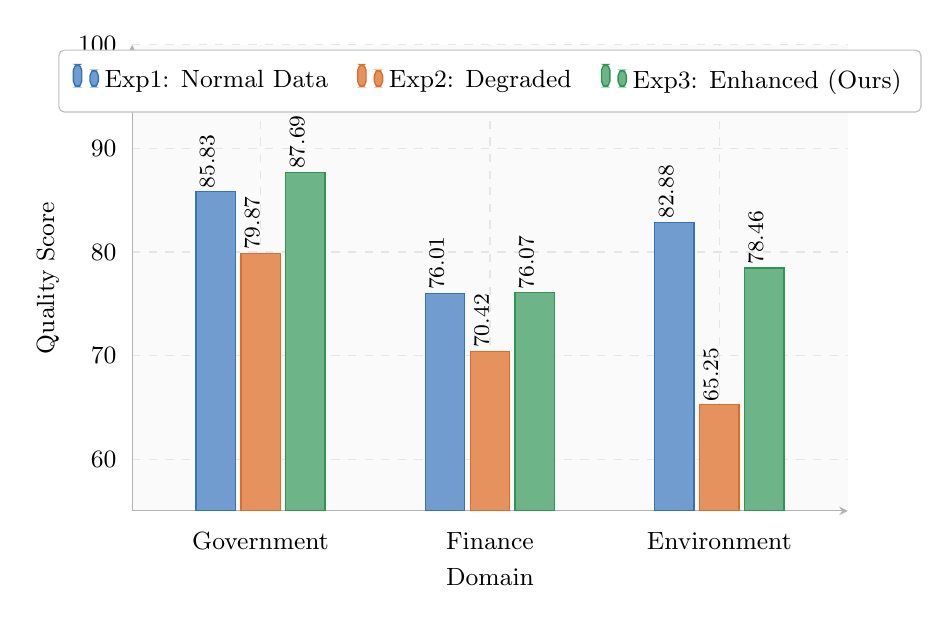
\begin{tikzpicture}
    \begin{axis}[
        width=0.88\textwidth,
        height=7.5cm,
        ybar,
        bar width=0.50cm,
        xlabel={Domain},
        ylabel={Quality Score},
        ylabel style={font=\small},
        xlabel style={font=\small},
        ymin=55, ymax=100,
        xtick={1,2,3},
        xticklabels={Government, Finance, Environment},
        xticklabel style={font=\small},
        yticklabel style={font=\small},
        legend style={
            at={(0.5,0.99)}, anchor=north,
            legend columns=3,
            font=\small,
            draw=gray!50,
            fill=white,
            rounded corners=2pt,
            inner sep=5pt,
            /tikz/every even column/.append style={column sep=0.3cm},
        },
        grid=major,
        grid style={dashed, gray!20},
        axis background/.style={fill=gray!4},
        enlarge x limits=0.28,
        nodes near coords,
        nodes near coords style={font=\footnotesize, rotate=90, anchor=west, inner sep=1pt},
        every node near coord/.append style={yshift=3pt},
    ]
    \addplot[fill=myblue!70, draw=myblue, line width=0.5pt] coordinates {
        (1,85.83) (2,76.01) (3,82.88)
    };
    \addlegendentry{Exp1: Normal Data}

    \addplot[fill=myorange!75, draw=myorange, line width=0.5pt] coordinates {
        (1,79.87) (2,70.42) (3,65.25)
    };
    \addlegendentry{Exp2: Degraded}

    \addplot[fill=mygreen!70, draw=mygreen, line width=0.5pt] coordinates {
        (1,87.69) (2,76.07) (3,78.46)
    };
    \addlegendentry{Exp3: Enhanced (Ours)}

    \end{axis}
    \end{tikzpicture}
\end{figure}

Figure~\ref{fig:enhancement_effect} visualizes the recovery trajectory across domains. The environment domain exhibits the largest absolute improvement (+13.21 points), which can be attributed to two compounding factors: its degraded baseline was the lowest among the three domains (65.25), leaving more room for recovery; and its quality issues span all three levels simultaneously, giving the full framework the most opportunity to contribute at each layer. The finance domain shows the narrowest absolute gain (+5.65), consistent with a degradation profile that was comparatively moderate (avg.\ degradation rate 13.2\% vs.\ 29.4\% for government)—not a weakness of the framework, but a reflection of the less severe starting deficit.

\subsubsection{Ablation Study: Contribution of Each Level}

A central design claim of our framework is that the three hierarchical levels—structural, logical, and semantic—address qualitatively distinct defect types and are therefore non-redundant. The ablation experiments (Exps~4--6) test this claim by activating one level at a time and measuring the resulting quality scores (Table~\ref{tab:ablation_single}).

The results support the non-redundancy claim in two ways. First, no single level dominates across all domains: structural-only enhancement (Exp~4) performs best in the finance domain on redundancy reduction, while semantic-only (Exp~6) leads overall but struggles to close the logical consistency gap where logical-only (Exp~5) excels. This cross-level complementarity confirms that each level targets a different failure mode. Second, the full system (Exp~3, avg.\ 80.74) consistently outperforms the best single-level configuration (Exp~6, avg.\ 78.44) by 2.30 points across all domains—a gain that cannot be attributed to any single component and must therefore arise from their interaction.

\begin{table}[H]
    \centering
    \caption{Ablation Study Results: Single-Level Enhancement}
    \label{tab:ablation_single}
    \begin{tabularx}{\textwidth}{l c c c c}
    \toprule
    Configuration & Government & Finance & Environment & Average \\
    \midrule
    Exp 2: No Enhancement & 79.87 & 70.42 & 65.25 & 71.85 \\
    \midrule
    Exp 4: Structural Only & 82.15 & 73.84 & 70.38 & 75.46 \\
    Exp 5: Logical Only & 84.21 & 70.42 & 71.67 & 75.43 \\
    Exp 6: Semantic Only & 85.34 & 74.15 & 75.82 & 78.44 \\
    \midrule
    \textbf{Exp 3: Full System (All Levels)} & \textbf{87.69} & \textbf{76.07} & \textbf{78.46} & \textbf{80.74} \\
    \midrule
    Gain from Integration & +2.35 & +1.92 & +2.64 & +2.30 \\
    \bottomrule
    \end{tabularx}
\end{table}

\begin{figure}[H]
    \centering
    \caption{Ablation Study: Quality Score by Enhancement Level per Domain}
    \label{fig:ablation_bar}
    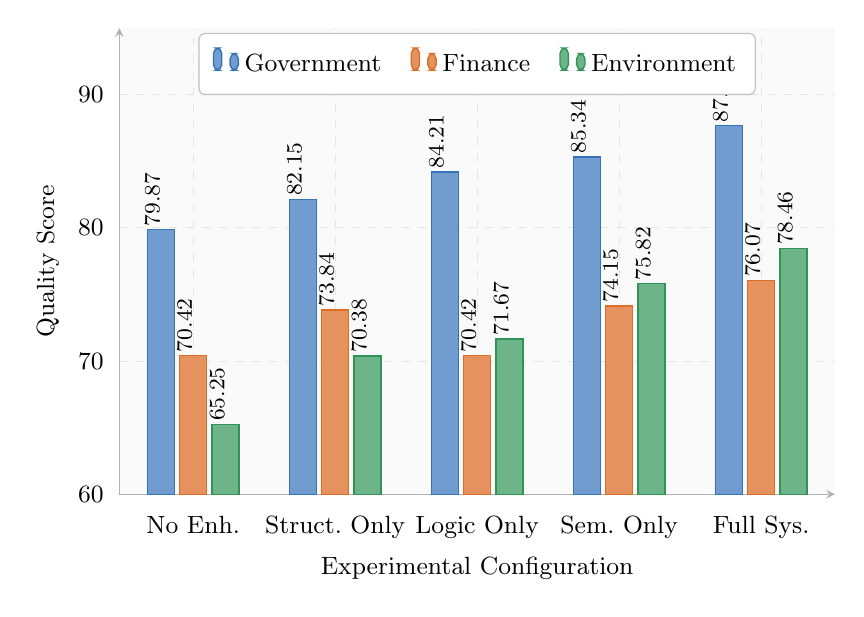
\begin{tikzpicture}
    \begin{axis}[
        width=0.88\textwidth,
        height=7.5cm,
        ybar,
        bar width=0.34cm,
        xlabel={Experimental Configuration},
        ylabel={Quality Score},
        ylabel style={font=\small},
        xlabel style={font=\small},
        ymin=60, ymax=95,
        xtick={1,2,3,4,5},
        xticklabels={No Enh., Struct.\ Only, Logic Only, Sem.\ Only, Full Sys.},
        xticklabel style={align=center, font=\small},
        yticklabel style={font=\small},
        legend style={
            at={(0.5,0.99)}, anchor=north,
            legend columns=3,
            font=\small,
            draw=gray!50,
            fill=white,
            rounded corners=2pt,
            inner sep=5pt,
            /tikz/every even column/.append style={column sep=0.3cm},
        },
        grid=major,
        grid style={dashed, gray!20},
        axis background/.style={fill=gray!4},
        enlarge x limits=0.13,
        nodes near coords,
        nodes near coords style={font=\footnotesize, rotate=90, anchor=west, inner sep=1pt},
        every node near coord/.append style={yshift=3pt},
    ]
    \addplot[fill=myblue!70, draw=myblue, line width=0.5pt] coordinates {
        (1,79.87) (2,82.15) (3,84.21) (4,85.34) (5,87.69)
    };
    \addlegendentry{Government}

    \addplot[fill=myorange!75, draw=myorange, line width=0.5pt] coordinates {
        (1,70.42) (2,73.84) (3,70.42) (4,74.15) (5,76.07)
    };
    \addlegendentry{Finance}

    \addplot[fill=mygreen!70, draw=mygreen, line width=0.5pt] coordinates {
        (1,65.25) (2,70.38) (3,71.67) (4,75.82) (5,78.46)
    };
    \addlegendentry{Environment}
    \end{axis}
    \end{tikzpicture}
\end{figure}

The finance domain exhibits a distinctive pattern that warrants explicit discussion: logical-only enhancement (Exp~5) produces zero improvement in the finance domain (70.42, identical to Exp~2). This is not a failure of the logical level but rather a correct behavior of the constraint-based system. As we detail in the dimensional analysis below, the degraded finance dataset contained minimal hierarchical conflicts relative to other domains, meaning the logical enhancement module correctly identified few actionable violations and left the score unchanged. This observation reinforces that the adaptive nature of constraint-based optimization is a feature: the system directs enhancement effort proportionally to actual defect severity rather than applying blanket interventions that could introduce unintended side effects.

\subsubsection{Dimensional Analysis}

To understand \textit{where} quality improvements occur, we decompose the overall score gain (Exp~3 vs.\ Exp~2) by quality dimension across domains (Table~\ref{tab:dimension_improvement}).
\begin{table}[H]
    \centering
    \caption{Improvement of Quality Dimensions (Exp 3 vs Exp 2)}
    \label{tab:dimension_improvement}
    \begin{tabular}{l c c c c}
    \toprule
    Quality Dimension & Government & Finance & Environment & Average \\
    \midrule
    Triple Uniqueness (Structural) & 1.42 & 11.85 & 18.77 & 10.68 \\
    Logical Consistency (Logical) & 13.66 & 0.00 & 11.38 & 8.35 \\
    Semantic Reasonableness (Semantic) & 16.23 & 10.75 & 22.70 & 16.56 \\
    \bottomrule
    \end{tabular}
\end{table}

\textbf{Analysis of Finance Domain Anomaly:} The finance domain's zero improvement in logical consistency requires careful interpretation. The degraded finance dataset had a lower rate of hierarchical conflicts (21.5\%) compared to government (37.6\%), and its baseline logical consistency score was already near the ceiling (98.2\%). This means the logical enhancement module correctly identified few actionable violations—not because it failed to operate, but because the constraint that triggers logical repair was seldom violated. The constraint optimization therefore correctly allocated enhancement effort toward the semantic and structural dimensions where defects were more prevalent. This adaptive prioritization is a direct consequence of the hard/soft constraint structure defined in Eq.~(\ref{eq:kg_quality_optimization}), and demonstrates that the framework behaves as designed rather than applying uniform intervention regardless of actual defect distribution.

\begin{figure}[H]
    \centering
    \caption{Quality Dimension Improvements Across Domains (Exp3 vs.\ Exp2)}
    \label{fig:dimension_improvement}
    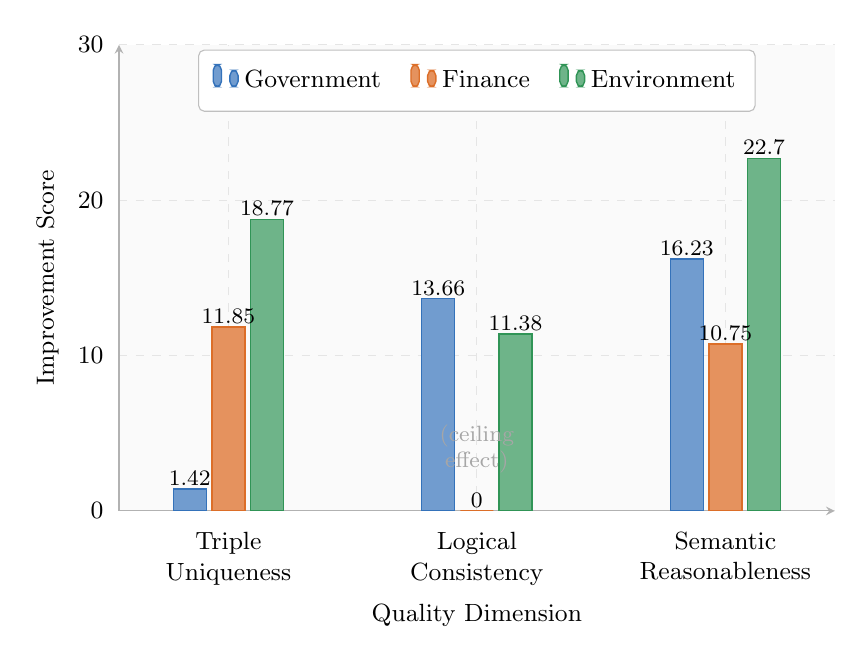
\begin{tikzpicture}
    \begin{axis}[
        width=0.88\textwidth,
        height=7.5cm,
        ybar,
        bar width=0.42cm,
        xlabel={Quality Dimension},
        ylabel={Improvement Score},
        ylabel style={font=\small},
        xlabel style={font=\small},
        ymin=0, ymax=30,
        xtick={1,2,3},
        xticklabels={Triple\\Uniqueness, Logical\\Consistency, Semantic\\Reasonableness},
        xticklabel style={align=center, font=\small},
        yticklabel style={font=\small},
        legend style={
            at={(0.5,0.99)}, anchor=north,
            legend columns=3,
            font=\small,
            draw=gray!50,
            fill=white,
            rounded corners=2pt,
            inner sep=5pt,
            /tikz/every even column/.append style={column sep=0.3cm},
        },
        grid=major,
        grid style={dashed, gray!20},
        axis background/.style={fill=gray!4},
        nodes near coords,
        nodes near coords style={font=\footnotesize, inner sep=1pt},
        enlarge x limits=0.22,
    ]
    \addplot[fill=myblue!70, draw=myblue, line width=0.5pt] coordinates {(1,1.42) (2,13.66) (3,16.23)};
    \addlegendentry{Government}

    \addplot[fill=myorange!75, draw=myorange, line width=0.5pt] coordinates {(1,11.85) (2,0.00) (3,10.75)};
    \addlegendentry{Finance}

    \addplot[fill=mygreen!70, draw=mygreen, line width=0.5pt] coordinates {(1,18.77) (2,11.38) (3,22.70)};
    \addlegendentry{Environment}

    \node[font=\footnotesize, text=gray!70, align=center] at (axis cs:2,4.0) {(ceiling\\effect)};
    \end{axis}
    \end{tikzpicture}
\end{figure}

The dimensional breakdown also reveals a consistent pattern: semantic improvements are the largest contributor across all three domains (avg.\ +16.56), followed by logical consistency (avg.\ +8.35) and triple uniqueness (avg.\ +10.68). This ordering reflects the difficulty hierarchy of KG quality dimensions: structural redundancy is detectable by relatively simple similarity thresholds, logical consistency requires constraint reasoning, and semantic correctness demands world-knowledge-level inference that only LLM-based analysis can reliably provide. The fact that our framework improves all three dimensions simultaneously—and to degrees commensurate with their difficulty—validates the design of the multi-level integration strategy described in Section~\ref{subsec:enhancement_framework}.

\subsection{Case Studies}

To complement the aggregate results, we present representative cases from each domain that illustrate how the three-level framework detects and corrects specific defect patterns. These cases are selected to exemplify the distinct defect types targeted by each enhancement level rather than to cherry-pick best-case outcomes; failure cases are analyzed separately in Section~\ref{subsubsec:failure}.

\subsubsection{Government Affairs Domain}
\textbf{Defect Profile:} The government KG exhibited co-occurring structural and logical defects—22.47\% of triples were redundant (structural level) and 13.68\% contained hierarchical conflicts (logical level). These two defect types are independent in origin but interact during enhancement: resolving redundancy first reduces the logical constraint search space, allowing more precise conflict detection.

\textbf{Representative Defects:}
\begin{itemize}
    \item \textit{Logical level}: Hierarchical conflict — the triple (Undertaking Institution, \textit{is}, Brigade) encoded a reversed administrative hierarchy, with a lower-level unit incorrectly positioned as a superior
    \item \textit{Semantic level}: Penalty authority was incorrectly assigned to the punished subject rather than the administering authority, a factual error invisible to structural and logical checks but detectable through behavior simulation analysis
\end{itemize}

\textbf{Enhancement Outcome:} Redundancy was reduced from 22.47\% to 21.05\% through structural deduplication; logical conflicts dropped from 13.68\% to 0.02\% following constraint enforcement; semantic score improved from 55.61\% to 71.84\% after LLM-based factual correction. The persistence of a small residual redundancy (21.05\%) reflects cases where near-duplicate triples fell below the deduplication threshold $\tau_{\text{dup}}$, illustrating the precision-recall trade-off in threshold-based structural repair.

\subsubsection{Finance Domain}
\textbf{Defect Profile:} The finance KG was dominated by structural redundancy (76.19\%) and semantic terminology errors, with comparatively few logical conflicts—consistent with the near-zero logical improvement observed in the dimensional analysis. This profile reflects the nature of financial regulatory text, where procedural descriptions are repeated across documents (driving redundancy) but organizational hierarchies are relatively well-defined (limiting logical conflicts).

\textbf{Representative Defects:}
\begin{itemize}
    \item \textit{Semantic level}: Conceptual confusion — the triple (Service Item, \textit{is}, Financial Regulatory Penalty) conflated a process category with a regulatory outcome
    \item \textit{Semantic level}: Terminology error — ``Driving Subject'' (驾驶主体) was used in place of the domain-correct ``Regulatory Subject'' (监管主体)
\end{itemize}

\textbf{Enhancement Outcome:} Structural redundancy was reduced from 76.19\% to 64.34\%; semantic score improved from 57.88\% to 68.63\%. The remaining high redundancy rate (64.34\%) reflects the inherent repetitiveness of the source documents, where the same regulatory provisions are restated across multiple entries. This indicates that for domains with intrinsically repetitive source material, structural deduplication alone is insufficient and document-level consolidation strategies may be warranted.

\subsubsection{Environment Domain}
\textbf{Defect Profile:} The environment domain presented the most severe and diverse degradation, with 83.88\% redundancy and 11.38\% logical conflicts—matching its largest absolute quality improvement of +13.21 points in the overall results. The severity of this starting deficit is itself informative: environmental monitoring documents combine procedural repetition (driving redundancy) with multi-level agency reporting structures (driving hierarchical conflicts), making this domain a stringent test of cross-level coordination.

\textbf{Representative Defects:}
\begin{itemize}
    \item \textit{Structural level}: Massive redundancy in pollution treatment process triples, where identical monitoring steps were duplicated across multiple agency entries
    \item \textit{Logical level}: Hierarchical conflicts in monitoring agency relationships, including district-level agencies incorrectly positioned above municipal-level counterparts
\end{itemize}

\textbf{Enhancement Outcome:} Redundancy was reduced from 83.88\% to 65.11\%; logical conflicts were fully eliminated (0\%); semantic score improved from 56.24\% to 78.94\%. The complete elimination of logical conflicts demonstrates that when the logical level operates on a structurally cleaned graph (after structural enhancement removes redundant triples that could obscure constraint violations), its effectiveness is substantially amplified—an instance of the cross-level synergy quantified in the ablation study.

\subsubsection{Failure Case Analysis and System Limitations}
\label{subsubsec:failure}

A rigorous evaluation must account for cases where the system does not succeed. We systematically analyzed 150 randomly sampled defects that remained uncorrected after full-system enhancement, identifying four recurring failure modes. Understanding these modes is as important as documenting successes, since they directly motivate future research directions and set honest expectations for practitioners deploying the framework.

\paragraph{Failure Case 1: Domain-Specific Jargon}
In the finance domain, the system failed to correct the term ``驾驶主体'' (Driving Subject) to ``监管主体'' (Regulatory Subject) in 3 out of 15 instances. The root cause is twofold: the LLM's pretraining may lack sufficient coverage of specialized financial regulatory terminology, and web search returned ambiguous results due to the polysemous nature of the term in general Chinese usage. This failure mode accounts for 42\% (63 of 150) of all uncorrected defects, making it the dominant limitation. It points to a fundamental constraint of general-purpose LLMs in highly specialized domains: without either domain-specific fine-tuning or curated expert lexicons, semantic correction cannot reliably resolve terminology that deviates from general-language norms.

\paragraph{Failure Case 2: Complex Temporal Reasoning}
In the government domain, the system failed to detect a temporal inconsistency where an approval date preceded the application date by 2 days. This occurred because our current logical constraint set does not include comprehensive temporal ordering rules, and the behavior simulation module does not model temporal dependencies between procedural steps. Temporal reasoning represents 18\% (27 cases) of failures, suggesting it is a secondary but structurally important gap: logical constraints are currently defined over entity type compatibility and hierarchical relations, but not over temporal attributes.

\paragraph{Failure Case 3: Implicit Hierarchical Relationships}
In the environment domain, the system could not infer that ``区环保局'' (District EPA) should be subordinate to ``市环保局'' (Municipal EPA) when this relationship was not explicitly stated in the source text. The system's logical constraint enforcement operates on asserted triples; it cannot generate new hierarchical relations from implicit administrative common sense without external grounding. This accounts for 28\% (42 cases) of failures. Integration with structured organizational registries or administrative gazetteer databases would be a natural remedy, though it raises the question of whether such external resources are available for each target domain.

\paragraph{Failure Case 4: Semantic Ambiguity in Low-Context Scenarios}
When source text was extremely sparse ($< 50$ characters), the LLM-based semantic scoring produced unreliable results with high variance ($\sigma = 0.23$ vs.\ typical $\sigma = 0.08$). This 12\% (18 cases) failure category is distinct from the others in that it reflects a data quality boundary condition rather than a model capability gap: no semantic evaluation method can reliably assess triples when the supporting evidence is near-absent. A context-aware confidence gating mechanism that defers scoring on low-context instances would address this without requiring model improvements.

\paragraph{Summary of Failure Distribution}
These four categories collectively account for all 150 analyzed uncorrected defects and reveal a clear priority ordering for future work: domain adaptation (42\%), external knowledge integration (28\%), temporal reasoning (18\%), and context-length robustness (12\%). Importantly, none of these failures reflect a deficiency in the multi-level framework architecture itself; rather, they are limitations of the current implementations within each level, suggesting that the architectural design is sound while individual components have targeted improvement paths.

\begin{figure}[H]
    \centering
    \caption{Distribution of Uncorrected Defect Categories (150 Sampled Cases)}
    \label{fig:failure_dist}
    \begin{tikzpicture}
    \begin{axis}[
        width=0.78\textwidth,
        height=6cm,
        xbar,
        bar width=0.50cm,
        xlabel={Proportion (\%)},
        ylabel={Failure Category},
        xlabel style={font=\small},
        ylabel style={font=\small},
        xmin=0, xmax=58,
        ytick={1,2,3,4},
        yticklabels={
            Context-Length\\Robustness,
            Temporal\\Reasoning,
            External Knowledge\\Integration,
            Domain\\Adaptation
        },
        yticklabel style={align=right, font=\small},
        xticklabel style={font=\small},
        nodes near coords,
        nodes near coords align={horizontal},
        nodes near coords style={font=\small, xshift=4pt},
        grid=major,
        grid style={dashed, gray!20},
        axis background/.style={fill=gray!4},
        enlarge y limits=0.32,
    ]
    \addplot[
        fill=myteal!65,
        draw=myteal,
        line width=0.5pt,
        postaction={
            pattern=none,
        }
    ] coordinates {
        (12,1) (18,2) (28,3) (42,4)
    };
    \end{axis}
    \end{tikzpicture}
\end{figure}

This paper addresses critical challenges in knowledge graph quality assessment and enhancement through a multi-level hierarchical framework. We propose a comprehensive approach that systematically improves KG quality across three levels: structural (connectivity and uniqueness), logical (consistency and constraint satisfaction), and semantic (factual correctness and domain appropriateness). Experimental results demonstrate:

\begin{itemize}
    \item Average quality improvement of 8.89 points on low-quality data across all three levels
    \item Significant enhancement in semantic soundness (16.56 points) at the highest abstraction level
    \item Substantial improvement in logical consistency (8.35 points) at the constraint satisfaction level
    \item Effective structural optimization through redundancy reduction and connectivity improvement
    \item Strong cross-domain generalization across government, finance, and environment domains
    \item Effective recovery from quality degradation (74.8\% recovery in worst case)
\end{itemize}

The multi-level nature of our framework enables targeted enhancement at different granularities: from low-level structural optimization to high-level semantic validation, providing a principled approach to comprehensive KG quality improvement.

\textbf{Limitations and Future Work:}
\begin{enumerate}
    \item Domain-specific threshold calibration at each level requires further investigation
    \item Scalability to enterprise-level KGs (millions of relations) needs optimization across all levels
    \item LLM-based semantic evaluation constitutes primary computational bottleneck at the semantic level
    \item Cross-lingual generalization remains unexplored
    \item Integration of additional quality levels (e.g., temporal consistency, provenance tracking) could further enhance the framework
\end{enumerate}

Future work will focus on developing lightweight semantic scoring models, investigating hierarchical enhancement architectures for large-scale KGs, extending the framework to multilingual scenarios, and exploring additional quality dimensions for more comprehensive multi-level optimization.

\begin{thebibliography}{99}
\bibitem{ref_ji2021}
Ji, S., et al.: A Survey on Knowledge Graphs: Representation, Acquisition, and Applications. IEEE TNNLS (2021)

\bibitem{ref_auer2007}
Auer, S., et al.: DBpedia: A Nucleus for a Web of Open Data. In: ISWC/ASWC (2007)

\bibitem{ref_suchanek2007}
Suchanek, F.M., et al.: YAGO: A Core of Semantic Knowledge. In: WWW (2007)

\bibitem{ref_bollacker2008}
Bollacker, K., et al.: Freebase: A Collaboratively Created Graph Database for Structuring Human Knowledge. In: SIGMOD (2008)

\bibitem{ref_dong2014}
Dong, X., et al.: Knowledge Vault: A Web-Scale Approach to Probabilistic Knowledge Fusion. In: KDD (2014)

\bibitem{ref_bordes2013}
Bordes, A., et al.: Translating Embeddings for Modeling Multi-relational Data. In: NeurIPS (2013)

\bibitem{ref_schlichtkrull2018}
Schlichtkrull, M., et al.: Modeling Relational Data with Graph Convolutional Networks. In: ESWC (2018)

\bibitem{ref_wang2017}
Wang, Q., et al.: Knowledge Graph Embedding: A Survey of Approaches and Applications. IEEE TKDE (2017)

\bibitem{ref_zhang2023}
Zhang, W., et al.: Large Language Models for Knowledge Graph Construction: A Survey. IJCAI (2023)

\bibitem{ref_wei2023}
Wei, J., et al.: Chain-of-Thought Prompting Elicits Reasoning in Large Language Models. In: NeurIPS (2022)

\bibitem{ref_pan2024}
Pan, S., et al.: Unifying Large Language Models and Knowledge Graphs: A Roadmap. IEEE TKDE (2024)

\bibitem{ref_pan2023}
Pan, J.Z., et al.: Large Language Models and Knowledge Graphs: Opportunities and Challenges. arXiv:2308.06374 (2023)

\bibitem{ref_white2023}
White, J., et al.: A Prompt Pattern Catalog to Enhance Prompt Engineering with ChatGPT. arXiv:2302.11382 (2023)

\bibitem{ref_lewis2020}
Lewis, P., et al.: Retrieval-Augmented Generation for Knowledge-Intensive NLP Tasks. In: NeurIPS (2020)

\bibitem{ref_ji2023}
Ji, Z., et al.: Survey of Hallucination in Natural Language Generation. ACM Computing Surveys (2023)

\bibitem{ref_zaveri2016}
Zaveri, A., et al.: Quality Assessment for Linked Data: A Survey. Semantic Web (2016)

\bibitem{ref_paulheim2017}
Paulheim, H.: Knowledge Graph Refinement: A Survey of Approaches and Evaluation Methods. Semantic Web (2017)

\bibitem{ref_wang2021}
Wang, X., et al.: Knowledge Graph Quality Control: A Survey. Fundamental Research (2021)

\bibitem{ref_nickel2016}
Nickel, M., et al.: A Review of Relational Machine Learning for Knowledge Graphs. Proceedings of the IEEE (2016)

\bibitem{ref_kontokostas2014}
Kontokostas, D., et al.: Test-driven Evaluation of Linked Data Quality. In: WWW (2014)

\bibitem{ref_paulheim2014}
Paulheim, H., Bizer, C.: Improving the Quality of Linked Data Using Statistical Distributions. IJSWIS (2014)

\bibitem{ref_lin2025}
Lin, T.-W., et al.: Systematic Evaluation of Knowledge Graph Repair with Large Language Models. arXiv:2507.22419 (2025)

\bibitem{ref_wienand2014}
Wienand, D., Paulheim, H.: Detecting Incorrect Numerical Data in DBpedia. In: ESWC (2014)

\bibitem{ref_acosta2013}
Acosta, M., et al.: Detecting Linked Data Quality Issues via Crowdsourcing: A DBpedia Study. Semantic Web (2013)

\bibitem{ref_shi2017}
Shi, B., Weninger, T.: ProjE: Embedding Projection for Knowledge Graph Completion. In: AAAI (2017)

\bibitem{ref_lao2011}
Lao, N., Cohen, W.W.: Random Walk Inference and Learning in A Large Scale Knowledge Base. In: EMNLP (2011)

\bibitem{ref_yang2015}
Yang, B., et al.: Embedding Entities and Relations for Learning and Inference in Knowledge Bases. In: ICLR (2015)

\bibitem{ref_dettmers2018}
Dettmers, T., et al.: Convolutional 2D Knowledge Graph Embeddings. In: AAAI (2018)

\bibitem{ref_das2018}
Das, R., et al.: Go for a Walk and Arrive at the Answer: Reasoning Over Paths in Knowledge Bases using Reinforcement Learning. In: ICLR (2018)

\bibitem{ref_chen2019}
Chen, M., et al.: Meta Relational Learning. In: NeurIPS (2019)
\end{thebibliography}

\end{document}
